\chapter{Metodologia}
Este capítulo apresenta as ferramentas e algoritmos utilizados neste projeto tanto no processo de extração do conhecimento, quanto na visualização dos dados.
A primeira seção irá explicar como os dados estão disponíveis na API da Riot Games e de que informações eles carregam. A segunda clarifica como estes dados serão armazenadas.  A terceira fala de que maneira se processa os dados, verifica se os dados estão completos e armazena-os em um banco de dados.

\section{API}
A Riot Games, desenvolvedora e dono do jogo \textit{League of Legends}, fornece uma Interface de Programação de Aplicativos ( do inglês \textit{Application Programming Interface} ) ou chamado de API, para que terceiros consigam acessar dados sobre os jogos.

A Riot games disponibiliza o acesso as informações à patir da URL\footnote{http://developer.riotgames.com} de modo que é gerado uma chave válida por 1 ano para projetos cadastrados.
O acesso à essa API é por URL utilizando uma função disponível pela Riot Games. Neste trabalho, usaremos apenas a função \textit{MATCH-V3} que é uma função que retorna os dados de uma partida já terminada.

A função \textit{MATCH-V3} é disponibilizada publicamente pela Riot Games, retornando um conjunto de informações no formato JSON sobre a partida passada por parâmetro, quando essa partida existe. A Figura \ref{fig:match-v3} resume um exemplo de uso da função acessando a URL\footnote{https://br1.api.riotgames.com/lol/match/v3/matches/1381102031?api\_key=minhachave}, acessada em 21 de março de 2018 pelo autor, sendo que \(minhachave\) tem que ser substituída por uma chave privada válida.
\begin{figure}[H]
	\caption{Exemplo de retorno do uso da função \textit{MATCH-V3}. Sendo as informações divididas em informações da partida, informações dos times e informações dos participantes.}
	\begin{center}
		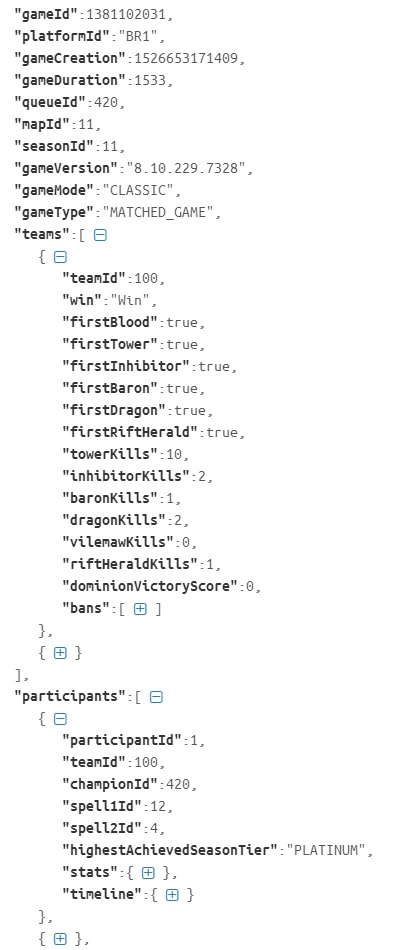
\includegraphics[width=9cm]{imagens/match-v3.jpg}
	\end{center}
	\small{Fonte: Autor.}
	\label{fig:match-v3}
\end{figure}

De todas essas informações retornadas pela função, as que foram armazenadas para o projeto por participante são:

\begin{enumerate}
\item \textit{gameId}. Identificador único da partida;
\item \textit{kills}, \textit{deaths} e \textit{assists}. Informações que falam, respectivamente, quantas vezes esse jogador matou, morreu e participou na morte de outrem;
\item \textit{win}. Se ele ganhou;
\item \textit{championId}. Qual campeão ele escolheu;
\item \textit{lane}. Em qual posição ele tava jogando;
\item \textit{platformId}. Em qual servidor ele jogava;
\item \textit{queueId}. E qual o tipo de partida.
\end{enumerate}

Sabendo qual informação vamos armazenar, ficou escolhido a linguagem \textit{Python} para ser desenvolvido o algoritmo no qual obterá as informações de forma não manual e o sistema de gerenciamento de banco de dados MySQL. Na próxima seção será apresentado sobre banco de dados e na seção \ref{section:get} será esclarecido como foram obtidos o \textit{dataset} das partidas. 


\section{Persistência dos dados}
Os dados adquiridos serão armazenados em um banco de dados MySQL, cujo o esquema das tabelas podem ser vistas na Figura \ref{fig:bd} onde é possível ver quais foram as informações salvas. Com o esquema do banco de dados pronto, já é possível passar para a aquisição dos dados.
\begin{figure}[H]
	\caption{Esquema usado do Banco de Dados.}
	\begin{center}
		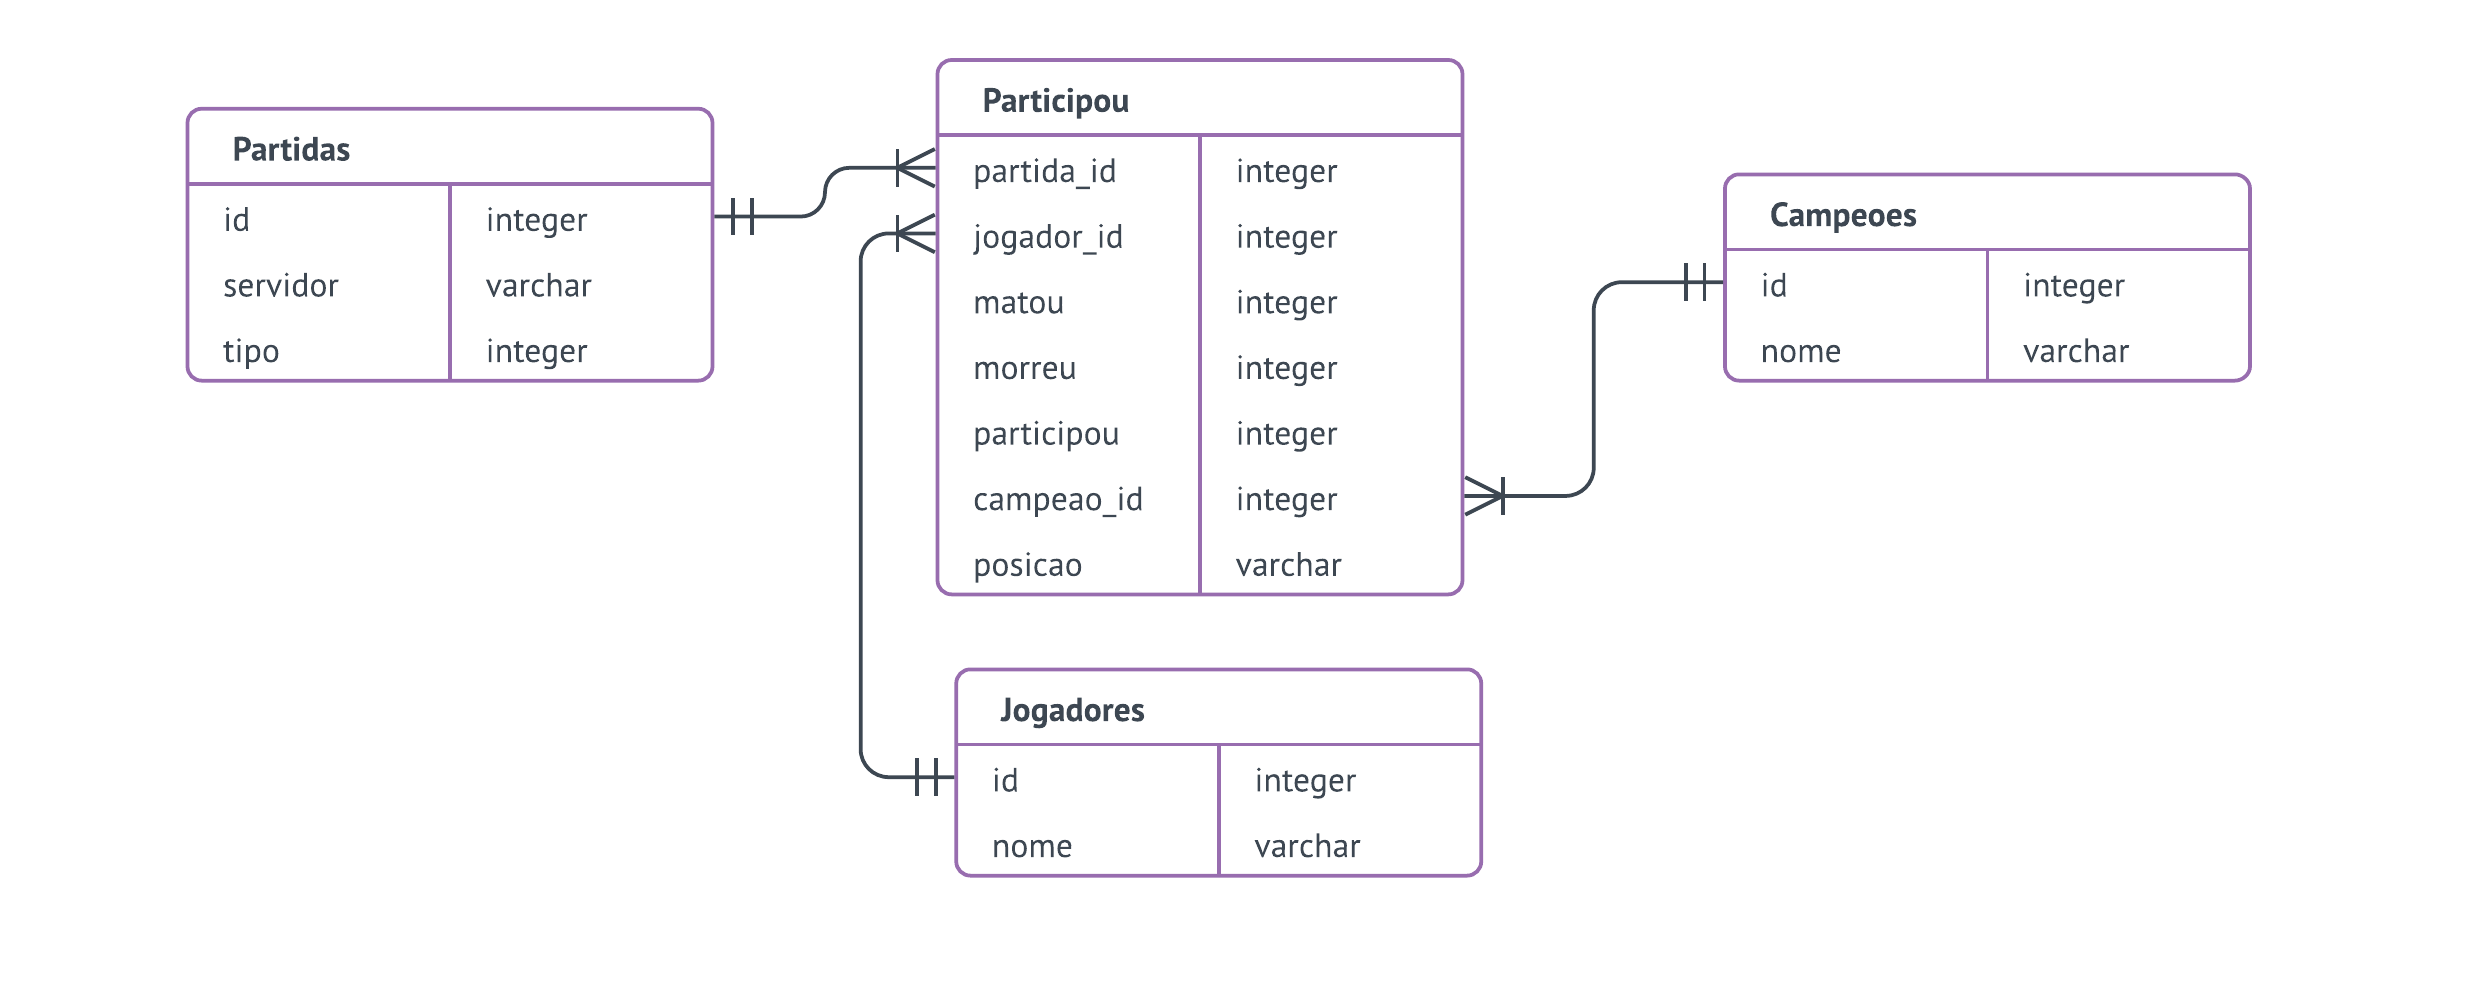
\includegraphics[width=17cm]{imagens/esquema.png}
	\end{center}
	\small{Fonte: Autor.}
	\label{fig:bd}
\end{figure}


\section{Aquisição dos dados}
A aquisição dos dados será dada à partir de duas fontes: A API da Riot Games e de um \textit{dataset} público\footnote{https://www.kaggle.com/paololol/league-of-legends-ranked-matches}. Ambos apresentam os mesmos conjuntos de informações em formatos diferentes. Será adquirido outros dados além destes que serão adquiridos pela API para agilização do trabalho.

A base de dados, na sua versão 9, conta com aproximadamente 183 mil partidas ranqueadas diferentes, dando uma incrementada no banco de dados inicialmente. Dados estes que precisam ser convertidos para o esquema do banco de dados usados no trabalho.

Depois, será usado um algoritmo para a aquisição dos dados de partidas pela API do \textit{League of Legends} em \textit{Python}, que usa a biblioteca \textit{requests} para conseguir acessar a API por URL's, verificando se a partida requisitada existe e se os dados necessários estão completos, salvando no banco de dados apenas as partidas válidas. O pseudo-código se encontra no Algoritmo \ref{alg:main-aqui}.

\
 %Código


\begin{algorithm}[H]
   \SetAlgoLined
     \Inicio{

		i = 1000000000;\tcp*[f]{Esta é a \textit{id} de uma partida aleatória na ultima versão do jogo}
            
		chave = minha chave privada de acesso;
            
        \uSe{Existe arquivo com ultimo partida lido}{
          	i = ultima partida lida;
        }
        \Repita{Até ser pausado}{    
            pedido = requisita URL Da API(i, chave);

            \Se((\tcp*[f]{Se a partida existe}){pedido.status == 200 }{
            	 
            	JSON = carrega JSON Do Pedido(pedido);
                
                \uSe{JSON é válido}{
                	Armazena os dados em um banco de dados;
                }
                
                i = i + 1;

            }
		}
	                
	Salva i no arquivo;
    }
   \label{alg:main-aqui}
   \caption{\textsc{Aquisição dos dados das partidas}}
 \end{algorithm}

\

Onde com esse algoritmo foram armazenadas \numpartidas\ jogos válidos diferentes, e foi decidido usar apenas as partidas ranqueadas 5 contra 5, já que estas são as partidas responsáveis pela classificação dos jogadores dentro dos jogo, e as partidas não ranqueadas são consideradas como amistosas.
Com esse escopo, o número de partidas usados foram ao todo \partidasrankeds\ partidas ranqueadas diferentes.
Na tabela \ref{tab:subset-lol} é possível ver uma pequena fatia dos dados salvos.


\begin{table}[H]
\centering
\caption{Exemplo de \textit{subset} salvo no banco de dados}
\label{tab:subset-lol}
\resizebox{\textwidth}{!}{%
\begin{tabular}{cccccccccc}
match\_id  & kills & deaths & assists & win & champ\_id & lane   & player\_id & platform & type \\
1282000002 & 11    & 10     & 7       & 0   & 67        & BOTTOM & 16112724   & BR1      & 420  \\
1282000002 & 2     & 8      & 15      & 0   & 412       & BOTTOM & 18604874   & BR1      & 420  \\
1282000002 & 7     & 4      & 7       & 0   & 34        & MIDDLE & 19281809   & BR1      & 420  \\
1282000002 & 7     & 6      & 4       & 0   & 5         & JUNGLE & 21304223   & BR1      & 420  \\
1282000002 & 5     & 7      & 12      & 0   & 98        & TOP    & 651014     & BR1      & 420  \\
1282000002 & 0     & 6      & 23      & 1   & 44        & BOTTOM & 18592234   & BR1      & 420  \\
1282000002 & 19    & 5      & 5       & 1   & 222       & BOTTOM & 7170345    & BR1      & 420 
\end{tabular}%
}
\small{Fonte: Autor.}
\end{table}

Na etapa seguinte são contabilizados quantas vezes cada campeão jogou com outro campeão, seja no mesmo time ou no time adversário, calculando quantas vitórias em oposição e quantas vitórias em junção.
E com as informações já processadas foi montado um \textit{web service}, que será explicado na seção \ref{chap:web}, utilizando uma biblioteca chamada D3.js para uma melhor visualização dos dados obtidos , biblioteca essa que será explanado na próxima seção.

\section{Visualização dos dados}
\label{chap:web}

O \textit{web service} foi criado utilizando o \textit{framework} Flask, que como \citet[tradução do autor]{flask} diz "Flask é um micro \textit{framework} para Python baseado em Werkzeug, Jinja 2 e em boas intenções.".

Com esse serviço será possível um relatório geral onde o usuário será capaz de ver a topologia do modelo, vendo quais são os campeões melhores contra os outros e quais são as duplas mais favoráveis, podendo filtrar quais campeões podem participar da pesquisa e quais não podem. 
Também será exequível a predição de uma partida, onde se seleciona os campeões de cada equipe e o sistema tenta antever quem vencerá.

Na Figura \ref{fig:web_service_relatorio} é possível ver um exemplo de uso do serviço para uma visão geral das informações. Na seção \ref{chap:pred} será esclarecido a maneira que essa predição da partida é feita.



\begin{figure}[H]
	
	\centering
	\caption{Exemplo de uso do \textit{web service} para visão geral dos dados.}
	\subfloat[Filtro dos dados para campeões da mesma equipe.]{
		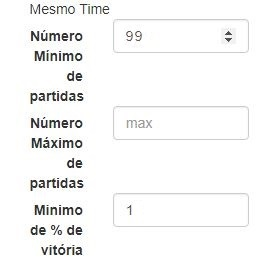
\includegraphics[width=0.4\textwidth]{imagens/web_1.JPG}
		}
	\subfloat[Filtro dos dados para adversários.]{
		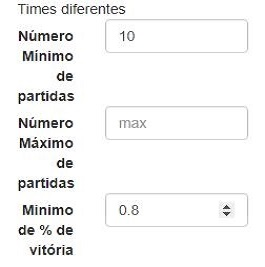
\includegraphics[width=0.4\textwidth]{imagens/web_2.JPG}
		}
	\qquad
	\subfloat[Filtro para escolher quais campeões podem participar (\textit{picks}) e quais nao podem (\textit{bans}).]{
		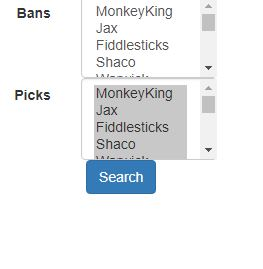
\includegraphics[width=0.4\textwidth]{imagens/web_3.JPG}
	}
	\subfloat[Exemplo de grafo exibido pelo \textit{web service}, sendo as setas vermelhas mostrando quem é bom contra quem, e as linhas continuas quem é bom com quem. O tamanho do circulo é a frequência daquela ligação e a cor é a força da ligação.]{
		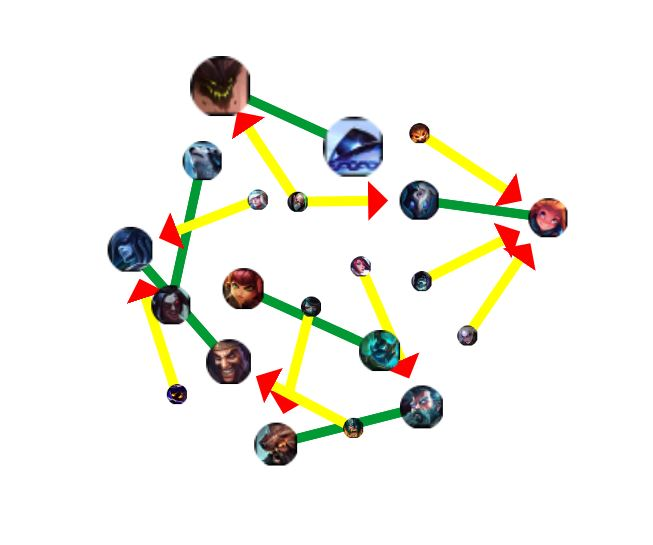
\includegraphics[width=0.4\textwidth]{imagens/web_4.JPG}
	}

	\small{Fonte: Autor.}
	\label{fig:web_service_relatorio}
\end{figure}


\section{Classificação da topologia}
Esperando o artigo.

\section{Predição dos dados}
\label{chap:pred}
Esperando as referencias.


\